\documentclass{tokaev-base}

\usepackage{tokaev-utils}
\usepackage{lipsum}
\usepackage{xstring}

\title{Laboratory work <<Theme>>}

\begin{document}

\maketitle
\section*{Purpose: }

\lipsum[1]

\section{Section 1}

\lipsum[1-2]

\section{Features}

\subsection[short]{Shortcuts}

Paste keys shortcuts inside text \Shortcut{keys for shortcut}.

\subsection[short]{Listings}

\subsubsection[short]{Inline listing}

Inline code listings \mintinline{html}{<h2>Something <b>here</b></h2>} with syntax highlightings.

\subsubsection[short]{Block listing}

\begin{minted}[]{c}
int main() {
    printf("hello, world");
    printf("hello, world");
    printf("hello, world");
    return 0;
}
\end{minted}

\section{Styled images and tables}

\subsection[short]{Images}

\begin{figure}[h]
    \centering
    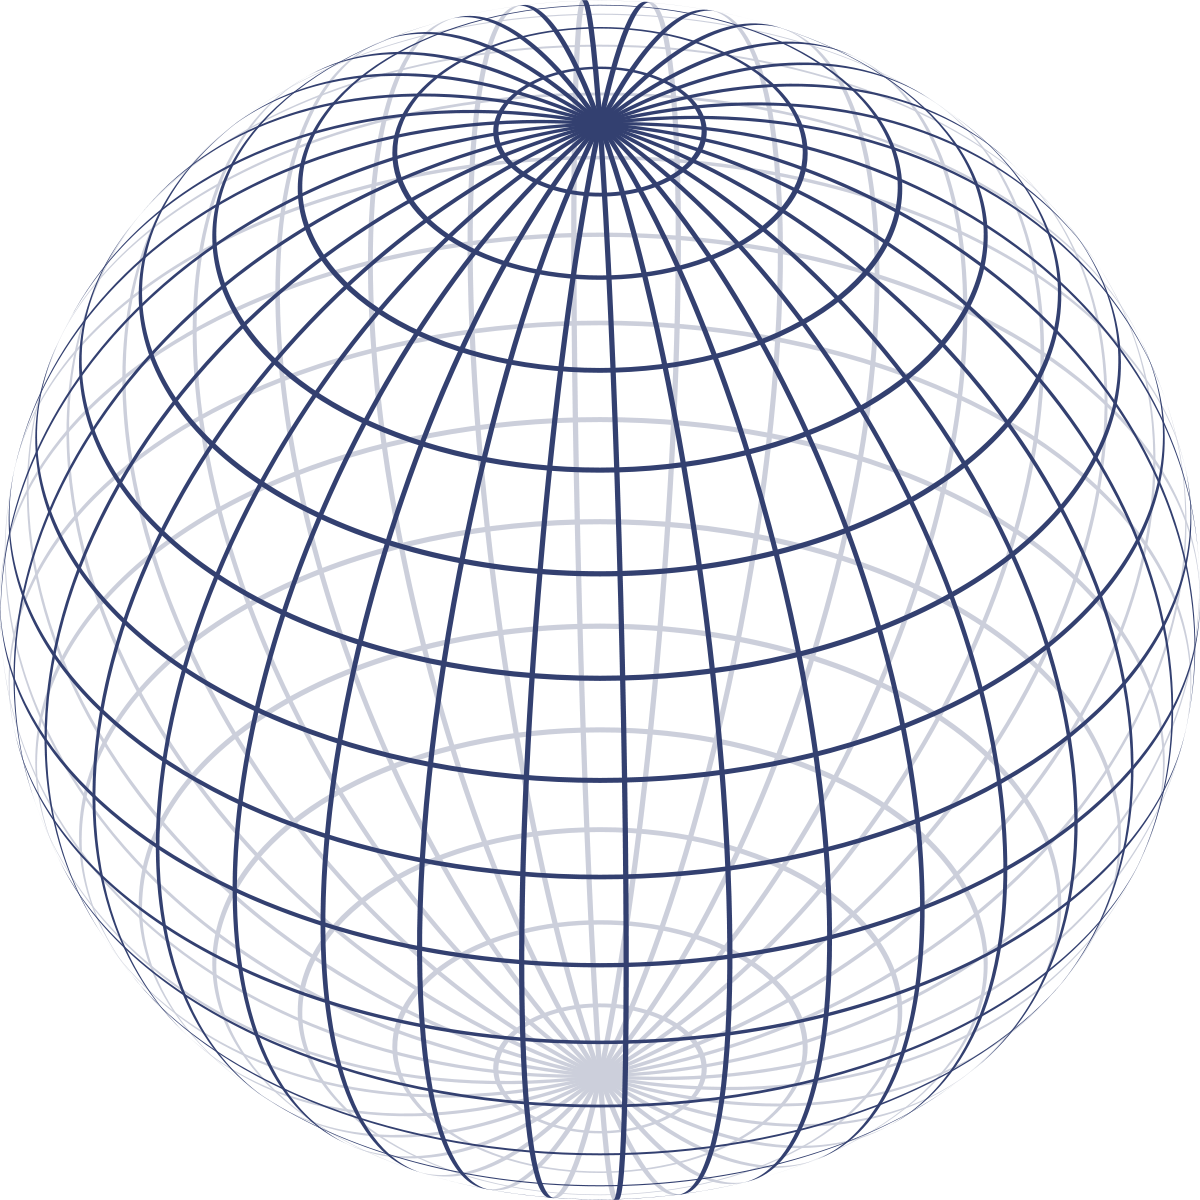
\includegraphics[width=0.4\textwidth]{image-example.png}
    \caption{image caption}
\end{figure}

\subsection[short]{Tables}

\begin{center}
    \begin{table}[h!]
        \caption{table caption}
        \centering
        \begin{tabular}{|c|c|}
            \hline
            Cell 1 & Cell 2 \\
            Cell 3 & Cell 4 \\
            \hline
        \end{tabular}
    \end{table}
\end{center}

\newpage

\section{Blank text section}

\subsection[short]{Blank text subsection}

\lipsum[1-4]

\end{document}
